\documentclass{mc2015}

%%%%%%%%%%%%%%%%%%%%%%%%%%%%%%%%%%%%%%%%%%%%%%%%%%%%%%%%%%%%%%%%%%%%%
\usepackage[T1]{fontenc}         % Use T1 encoding instead of OT1
\usepackage[utf8]{inputenc}      % Use UTF8 input encoding
\usepackage{microtype}           % Improve typography
\usepackage{booktabs}            % Publication quality tables
\usepackage{amsmath}
\usepackage{graphicx}
\usepackage{float}
\usepackage{wrapfig}
\usepackage[exponent-product=\cdot]{siunitx}
\usepackage[colorlinks,breaklinks]{hyperref}
\hypersetup{linkcolor=black, citecolor=black, urlcolor=black}

\usepackage{lipsum}
\usepackage{listings}
\lstset{language=C,frame=single,breaklines=true,backgroundcolor=\color{white},
	basicstyle=\ttfamily}

\def\equationautorefname{Eq.}
\def\figureautorefname{Fig.}

%%%%%%%%%%%%%%%%%%%%%%%%%%%%%%%%%%%%%%%%%%%%%%%%%%%%%%%%%%%%%%%%%%%%%
% Insert authors' names and short version of title in lines below

\authorHead{B.S. Cornille}
\shortTitle{Shared Memory MC}

%%%%%%%%%%%%%%%%%%%%%%%%%%%%%%%%%%%%%%%%%%%%%%%%%%%%%%%%%%%%%%%%%%%%%
\begin{document}

\title{Shared Memory Monte Carlo with MPI+MPI}

\author{Brian Cornille}
%\author{Author B\footnote{Footnote, if necessary}}
\affil{University of Wisconsin-Madison \\
%  1500 Engineering Dr. \\
%  Madison, WI 53706 \\
  bcornille@wisc.edu}

%\author{Author C}
%\affil{
%  Department of Nuclear Engineering \\
%  Name of University \\
%  Address \\
%  C@name.univ.edu
%}

\maketitle

\begin{abstract}



\emph{Key Words}: Monte Carlo, MPI+MPI
\end{abstract}

%%%%%%%%%%%%%%%%%%%%%%%%%%%%%%%%%%%%%%%%%%%%%%%%%%%%%%%%%%%%%%%%%%%%%
\section{Introduction}

The primary objective of this project was to demonstrate the feasibility of
shared memory tallies for Monte Carlo calculations using the MPI shared memory framework.
First, some motivation is given for the need for this type of system.
Then a brief description of the MPI functionality that enables this work is given,
followed by a the definition of the model problem that is used for testing code.
The source code for this project, including examples of the programming concepts used,
as well as this white paper can be found at
\url{https://github.com/bcornille/mpi-shared-ne506}
(currently residing in the \lstinline$rush$ branch;
it will eventually be incorporated into the \lstinline$master$ branch,
as this is an ongoing project).


\subsection{Motivation for Shared Memory}

Currently, extremely large Monte Carlo calculations may be carried out on
high performance computing (HPC) systems.
In most cases these codes are developed with distributed memory parallel capabilities
using the Message Passing Interface (MPI) standard.
Some of these may even use a hybrid parallel programming model,
such as MPI+OpenMP, in which MPI handles the parallelism at the HPC system level
and the second programming model handles parallelism at the compute node level.
This hybrid parallel programming model more closely resembles
the physical structure of an HPC system.
The lower level parallelism at the compute node level is done using shared memory.
When only MPI is used for parallelism in Monte Carlo codes,
the problem set-up must be repeated for each process.
This means that there may be many copies of the geometry and tallies
on a single compute node, which has one pool of shared memory.
This makes the hybrid parallel approach advantageous,
especially when the size of the geometry and tallies becomes prohibitively large
from a memory standpoint.
However, using two programming models to achieve a hybrid parallel code
can be difficult to implement.
Recent additions have been made to the MPI standard that allow it to implement
shared memory parallelism without the need for a second programming model.
This project attempt to produce a simplified Monte Carlo particle transport code
using an MPI+MPI hybrid parallel programming structure.

\subsection{Shared Memory Programming Considerations}

Programming with shared memory can have additional difficulties
compared to serial or distributed parallel programming.
With shared memory multiple processes or threads have access to the same memory locations.
Without proper precautions, there is risk of producing a \emph{race condition}.
A race condition is possible when multiple processes try to
update the same memory simultaneously.
This can produce inconsistent and unpredictable results.
Specific care must be taken to ensure that these types of errors do not occur.
Generally this is done by manual locking of the memory to prevent access
by more than one process or by specialized routines for updating memory.

\subsubsection{MPI\_Accumulate}

For Monte Carlo calculations a shared memory tally represents
a risk of having a race condition.
The tally requires consistent updating from contributions from
the independent streams of particle histories on each process.
The MPI-3.0 standard provides a routine that provides
the necessary functionality for updating tallies in a safe way.
This is the function \lstinline$MPI_Accumulate$.
The MPI standard defines the C binding for this function\cite{MPIbook}
\begin{lstlisting}
int MPI_Accumulate(const void *origin_addr, int origin_count,
    MPI_Datatype origin_datatype, int target_rank,
    MPI_Aint target_disp, int target_count,
    MPI_Datatype target_datatype, MPI_Op op, MPI_Win win);
\end{lstlisting}
Using this function each process will be able to post contributions to the tally.
The MPI standard guarantees that each posted \lstinline$MPI_Accumulate$ call
will update the target.
However, it does not guarantee the order that these postings will be executed.
For tallies only additive contributions from each particle history are produced,
thus the order of addition of those terms will not affect the result.

\subsection{Model Problem}

A very simple model problem was desired for this study.
Since no physics was to be tested, it was not necessary to model a
physically realistic test case.
The only requirement for the test problem was that an appropriate amount
of computation should be done between each particle transport step.

\subsubsection{Geometry}

%\begin{wrapfigure}{R}{0.47\textwidth}
\begin{figure}[h]
%	\vspace{-30pt}
	\centering
		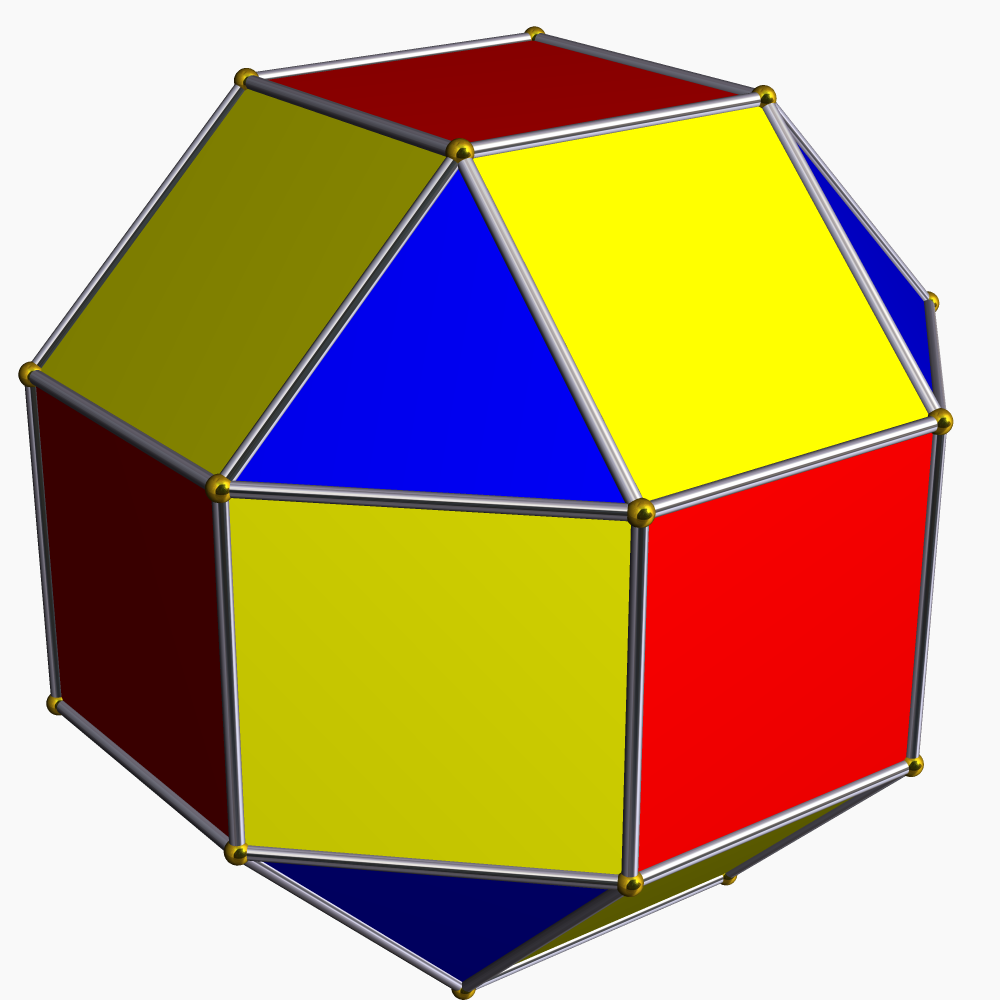
\includegraphics[width=0.35\textwidth]{Small_rhombicuboctahedron.png}
		\caption{\small "Small rhombicuboctahedron" by Tomruen -
			\url{http://en.wikipedia.org/wiki/Image:small_rhombicuboctahedron.png.}}
		\label{fig:shape}
%	\vspace{-20pt}
\end{figure}
%\end{wrapfigure}

The model geometry was chosen to be a single cell with the shape of a rhombicuboctahedron.
A rhombicuboctahedron has 26 faces,
of which 18 are square and 8 are equilateral triangles (see \autoref{fig:shape}).
This shape was chosen for having many unique bounding surfaces that are simple to define.
Having many bounding surfaces adds computation
when determining the next particle position.
This helps the model problem approximate the computational time
per particle transport step of a realistic case.
The rhombicuboctahedron used would contain an inscribed sphere of radius 1 unit.
Particle histories are terminated once they leave this cell.

\subsubsection{Material properties}

A made up material was created for the model problem.
This material has a particle mean free path of 0.1 units and produces
hard sphere collisions.
The material has no other properties that would affect the particle transport.

\noindent
\emph{Hard sphere collision derivation:}

Assuming even sampling on a circular cross section the circular coordinates can be sampled
\begin{subequations}
\begin{align}
	\rho &= \sqrt{\xi} \label{eq:rho}\\
	\phi &= 2\pi\eta \label{eq:phi1}
\end{align}
\end{subequations}
where $\rho$ is a normalized radius, and $\xi$ and $\eta$ are randomly sampled variables
on the domain $[0,1)$.
For a hard sphere, given a scattering angle $\theta$,
the normalized impact parameter can be shown to follow
\begin{equation}
	\rho(\theta) = \cos\left(\frac{\theta}{2}\right) \label{eq:impact}
\end{equation}
By solving for $\theta$ and substituting \autoref{eq:rho},
the random sampling of scattering angle in the particles coordinate frame is given by
\begin{subequations}
\begin{align}
	\theta &= 2\cos^{-1}\left(\sqrt{\xi}\right) \label{eq:theta}\\
	\phi &= 2\pi\eta \label{eq:phi2}
\end{align}
\end{subequations}
Once these two angles are determined,
a coordinate system can be generated based on the old particle flight direction.
Since the scattering is cylindrically symmetric, two of the axes of this system
are arbitrary as long as they are orthonormal to the old particle flight.
The scattered direction can then be simply transformed
back to the global coordinate frame via
\begin{equation}
	\bf{n} = \cos(\phi)\sin(\theta)\bf{e_1} + \sin(\phi)\sin(\theta)\bf{e_2}
			+ \cos(\theta)\bf{e_3}
\end{equation}
where $\bf{n}$ is the scattered direction and $(\bf{e_1},\bf{e_2},\bf{e_3})$
is the particle collision coordinate system,
with $\bf{e_3}$ being the pre-collision flight direction.

\subsubsection{Source}

A point source is used.
It originates at the point $(0,0,1)$ and is directed in the $(0,0,-1)$ direction.

\subsubsection{Tally}

The model problem includes a 3-D Cartesian mesh tally
that encapsulates the entire geometry.
The mesh is evenly spaced and with equal number of bins in each direction.
This number of bins can be adjusted as a runtime input parameter.

%%%%%%%%%%%%%%%%%%%%%%%%%%%%%%%%%%%%%%%%%%%%%%%%%%%%%%%%%%%%%%%%%%%%%
\section{Conclusions}

A simplistic Monte Carlo particle transport code was successfully made
and a shared memory tally was implemented.
Various test cases were run to investigate the implications
of a shared memory tally on program execution time.

\subsection{Resutls}

\begin{figure}[h]
	\centering
	\includegraphics[width=0.75\textwidth]{timings.pdf}
\end{figure}

%%%%%%%%%%%%%%%%%%%%%%%%%%%%%%%%%%%%%%%%%%%%%%%%%%%%%%%%%%%%%%%%%%%%%
\section{Acknowledgments}



%%%%%%%%%%%%%%%%%%%%%%%%%%%%%%%%%%%%%%%%%%%%%%%%%%%%%%%%%%%%%%%%%%%%%
\setlength{\baselineskip}{12pt}

\bibliographystyle{mc2015}
\bibliography{references}

%%%%%%%%%%%%%%%%%%%%%%%%%%%%%%%%%%%%%%%%%%%%%%%%%%%%%%%%%%%%%%%%%%%%%
%\appendix
%\section{}

\end{document}
